\documentclass[onecolumn, 11pt, draftclsnofoot]{IEEEtran}

\usepackage{epsfig,graphics,epsf,amsfonts,color,mathrsfs,amssymb,bm,caption,algorithm,algorithmic}
\usepackage{url}

\usepackage{amsmath}
\newcommand{\bsb}{\boldsymbol}
\newcommand{\mb}{\mathbf}
\newcommand{\mc}{\mathcal}
\newcommand{\mexpc}{\mathrm{E}}
\newcommand{\ve}{\mathrm{vec}}
\newcommand{\toep}{\mathcal{T}}
\newcommand{\tr}{\mathrm{tr}}
\newcommand{\tred}{\color{red}}
\textheight=9.2in
\DeclareCaptionLabelFormat{lc}{\MakeLowercase{#1}~#2}
\captionsetup{labelfont=sc,labelformat=lc}
\renewcommand{\figurename}{Figure}
\renewcommand{\theequation}{R\arabic{equation}}

\usepackage[numbers]{natbib}

%\hyphenation{op-tical net-works semi-conduc-tor}
\begin{document}
The authors appreciate the helpful comments and suggestions from both reviewers. 
Throughout this response letter, we will follow the following notational
rules for citations and references:
\begin{itemize}
  \item Citations: references in this response letter are cited with prefix
  ``R'' (e.g. [R 1]) whereas references in the original manuscript are cited
  without prefix (e.g. [1]).
  \item Equations: equations in this response letter are referred to as
  ``Eq.~(R1)''  while those in the original manuscript as ``Eq.~(1)''.
  \item Figures: figures in this response letter are referred to as
  ``FIGURE~1''  while those in the original manuscript as ``Fig.~1''.
\end{itemize}

\begin{center}
  {\LARGE \textbf{Authors' Response to Reviewer 1}}
\end{center}

% ~\citep[R][]{cheng2013thermal}
% \begin{align}
%   sfsdf
%   \label{eq:test}
% \end{align}
% \eqref{eq:test}
% \begin{figure}[!t]
%   \centering
%   \includegraphics[width=0.75\columnwidth]{./figs/test.eps}
%   \caption{Average throughput.}
%   \label{fig:test}
% \end{figure}
% Fig.~\ref{fig:test}

 
%%%%%%%%%%%%%%%%%%%%%%%%%%%%%%%%%%%%%%%%%%%%%%%%%%%%%%%%%%%%%%%%
\noindent
\emph{1. The novelty of this work may be limited by the simplicity of the model,
as it seems the method can only be applied when two RRHs cooperate. }

\noindent \textbf{Authors' response:} 
Indeed we assume for simplicity two RRHs in full
cooperation. But the concept we propoesd is applicable to a wide range of
scenarios and is scalable. First of all, cooperative transmission has both
attracted great research interest [10][11] and been incorporated into the latest
wireless communication systems such as LTE-advanced~\citep[R][]{TR36.819}. The
simplicity of this model allows its adoption in many practical scenarios, such as
joint transmission between different sectors/cells from a same macro base
station (BS), between homogeneous cells covered by a macro BS and its high-power RRHs, 
or between heterogeneous cells covered by a macro BS and its low-power RRHs, etc. Recent studies 
on Cloud Radio Access Network
(C-RAN)~\citep[R][]{6897914}\citep[R][]{6923535} have also promoted new network architectures where CoMP could find its application.
Consequently, we believe that cooperative RRHs is a simple yet practical and
meaningful setup, and, to the best of our knowledge, MoDiv design for improved performance has not
been studied under this scenario previously.

For cases involving $N>2$ cooperative RRHs, it is possible to
scale our MoDiv design approach into a quadratic $(N+1)$-dimensional
assignment problem at the cost of growing complexity. However, in reality,
the cluster size of CoMP is limited by backhaul link constraints or by the need for 
simple scheduler operation~\citep[R][]{6146494}. It is more
practical to utilize no more than two or three transmitters in cooperation
to serve one user equipment (UE) on cell/sector
edges~\citep[R][]{4385782, 5463229, 5456455} or in an overlaid heterogeneous
network~\citep[R][]{6879305, 6362916}. Furthermore, even in the cases of $N>2$, 
we can also group the $N$ RRHs into two groups to form two virtual RRHs with
multi-antennas to apply our MoDiv design directly for simplicity with little performance loss. 

In order to emphasize the generality of our system model, in the revised
manuscript, we have used cooperative ``transmitters'' instead of ``RRHs'' to
imply that our approach applies to a wider range of CoMP systems.

\vspace{0.5cm}

%%%%%%%%%%%%%%%%%%%%%%%%%%%%%%%%%%%%%%%%%%%%%%%%%%%%%%%%%%%%%%%%
\noindent
\emph{2. The signal model needs further work: $p$ is reported as “index” before
(1) and something to be demodulated in (3); in (1), which is the transmit
vector/symbol? }

\noindent \textbf{Authors' response:}
Thank you for the comment. As mentioned in the first paragraph in Section
II, the transmitted vector corresponding to two symbols are
$\bm{\psi}^{(m)}[p] = [\psi_1^{(m)}[p], \psi_2^{(m)}[p]]^T$, where
$p=0,\ldots,Q-1$ is the index/label corresponding to a bit sequence of length
$\log_2Q$, and in Eq.~(1) the transmitted symbols at the two RRHs are
$\psi_1^{(m)}[p]$ and $\psi_2^{(m)}[p]$, respectively. For instance, for 16-QAM where $Q=16$, in
one round of (re)transmission every 4 bits can be mapped to 2 constellation
symbols as in TABLE~\ref{table:mapping} and FIGURE~\ref{fig:mapping}.

Demodulation of the information bits is equivalent to determining label $p$ from
received signal $\mathbf{y}^{n}$ where $n=0,\ldots,m$ denote different
rounds of (re)transmissions. Since channel noise is Gaussian and we
assume known CSI at the receiver, the maximum-likelihood rule is in the form
of Eq.~(3).

To prevent possible confusion by our readers, we rephrase the description of
our signal model in the first paragraph of Section II, using similar
terminology as [4]. Most notably, we have renamed $p$ as ``label'', which is
commonly used in related works [4]\citep[R][]{1388738, 7494668}, instead of
``index'' throughout the manuscript.

\begin{table}[!t]
  \renewcommand{\arraystretch}{1.3}
  \caption{Mapping from bits to constellation symbols.}
  \label{table:mapping}
  \centering
  \begin{tabular}{c|c|c|c}
    \hline
     bits & $p$ & $\psi_1^{(m)}[p]$ & $\psi_2^{(m)}[p]$  \\
    \hline
    0000 & 0 & $-3+3j$ & $-1+1j$ \\
    0001 & 1 & $-3+1j$ & $-1-3j$ \\
    0010 & 2 & $-3-3j$ & $-1-1j$ \\
    0011 & 3 & $-3-1j$ & $-1+3j$ \\
    0100 & 4 & $-1+3j$ & $+3+1j$ \\
    0101 & 5 & $-1+1j$ & $+3-3j$ \\
    0110 & 6 & $-1-3j$ & $+3-1j$ \\
    0111 & 7 & $-1-1j$ & $+3+3j$ \\
    1000 & 8 & $+3+3j$ & $+1+1j$ \\
    1001 & 9 & $+3+1j$ & $+1-3j$ \\
    1010 & 10 & $+3-3j$ & $+1-1j$ \\
    1011 & 11 & $+3-1j$ & $+1+3j$ \\
    1100 & 12 & $+1+3j$ & $-3+1j$ \\
    1101 & 13 & $+1+1j$ & $-3-3j$ \\
    1110 & 14 & $+1-3j$ & $-3-1j$ \\
    1111 & 15 & $+1-1j$ & $-3+3j$ \\
    \hline
  \end{tabular}
\end{table}

\begin{figure}[htb]
  \begin{minipage}[b]{0.48\linewidth}
    \centering
    \centerline{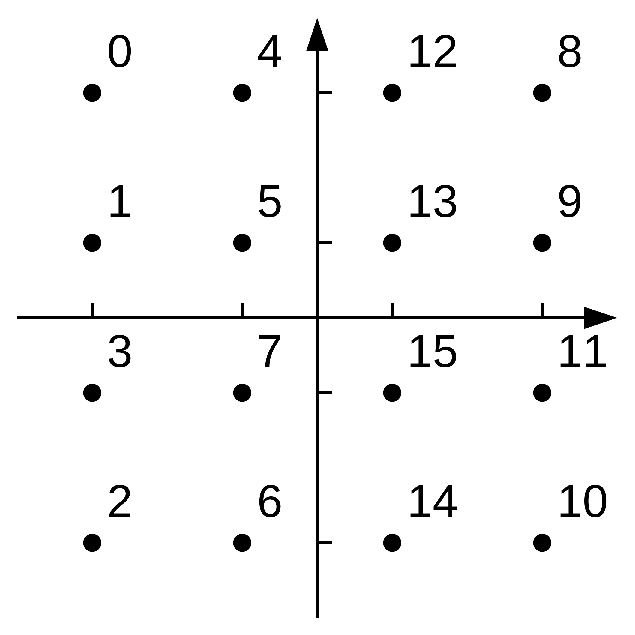
\includegraphics[width=4.0cm]{./figs/gray.eps}}
    \centerline{(a) $\psi_1^{(m)}[p]$ (Gray mapping)}\medskip
  \end{minipage}
  \hfill
  \begin{minipage}[b]{.48\linewidth}
    \centering
    \centerline{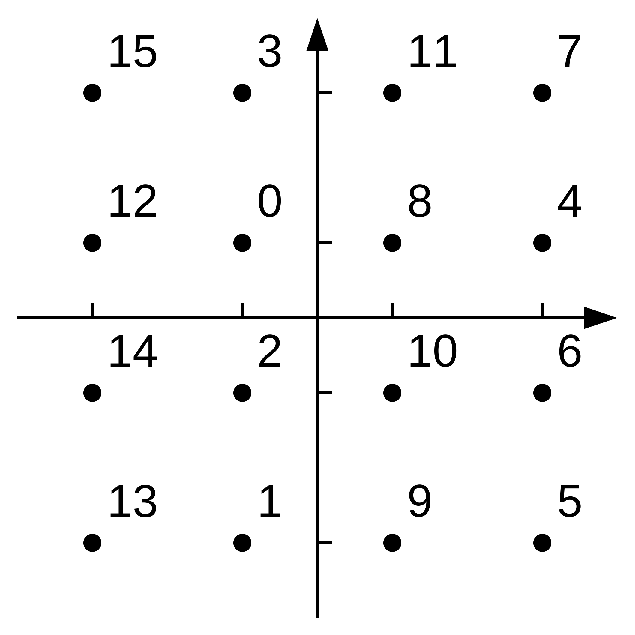
\includegraphics[width=4.0cm]{./figs/karim.eps}}
    \centerline{(b) $\psi_2^{(m)}[p]$ (trans-modulation design in [5])}\medskip
  \end{minipage}
  \caption{Constellation symbols. Label $p$ are marked next to each
  constellation symbol and we assume that the horizontal and vertical
  distances between two neighboring constellation symbols are both 2.}
  \label{fig:mapping}
\end{figure}
\vspace{0.5cm}

%%%%%%%%%%%%%%%%%%%%%%%%%%%%%%%%%%%%%%%%%%%%%%%%%%%%%%%%%%%%%%%%%
\noindent
\emph{3. Some more not defined expressions/symbols/variables: in (2),
$\bar{\mathbf{H}}_a$ (first term); CSCG.}

\noindent \textbf{Authors' response:}
Thank you for pointing out this ambiguity. We have added descriptions on
$\bar{\mathbf{H}}_a$ and used the common notation $\mathcal{CN}(0,1)$
in place of standard Circularly Symmetric Complex Gaussian (CSCG) following
Eq.~(2).

\vspace{0.5cm}

%%%%%%%%%%%%%%%%%%%%%%%%%%%%%%%%%%%%%%%%%%%%%%%%%%%%%%%%%%%%%%%%%%
\noindent
\emph{4. Proposition 1: the proof is abridged in excess. For instance, the
derivation of (9) is hard to understand.}

\noindent \textbf{Authors' response:}
Thank you for the comment. Due to the page limit of the IEEE Communications
Letters, we have no room to provide a full proof in the original manuscript. Thus, we
outline only the key steps. A rigorous proof of Proposition 1 is attached
in Appendix A in this response letter. We will provide online access to this proof as
supplementary material once our manuscript is accepted (because of the doubly-blind
journal policy). 
 
\vspace{0.5cm}

%%%%%%%%%%%%%%%%%%%%%%%%%%%%%%%%%%%%%%%%%%%%%%%%%%%%%%%%%%%%%%%%
\noindent
\emph{5. In Section III.B, the method has not been presented with sufficient
detail. Why do you introduce $x$ variables? What is the role of ``flow'' and
``distance'' matrices? How do you derive (13)?}

\noindent \textbf{Authors' response:}
Thank you for the question. The introduction of the variable $\mathbf{x}^{(m)}$
is to facilitate a standard representation of Q3AP formulation
[14]\citep[R][]{frieze1974bilinear}\citep[R][]{balas1991algorithm}\citep[R][]{burkard1999linear}\citep[R][]{5587019}.
In our problem, there is a one-to-one mapping between the 3-D permutation matrix
$\mathbf{x}^{(m)}\in\mathcal{S}$ (Eq.~(12)) and the vector mapping function
$\bm{\psi}^{(m)}[p] = [\psi_1^{(m)}[p], \psi_2^{(m)}[p]]$. 

The ``flow'' and ``distance'' matrices are terminologies borrowed from the
Koopmans-Beckmann form Quadratic Assignment Problem
(QAP)~\citep[R][]{koopmans1957assignment}\citep[R][]{806935}:
\begin{align}
  & \min_{\mathbf{x}}
  \sum_{p=1}^{n}\sum_{i=1}^{n}
  \sum_{q=1}^{n}\sum_{j=1}^{n}
  f_{pq}d_{ij}x_{pi}x_{qj},\notag\\
  \mbox{s.t. } & \sum_{p=1}^{n}x_{pi} =
  1,\sum_{i=1}^{n}x_{pi} = 1, x_{pi}\in\{0, 1\}
\end{align}
which is formulated from the following problem. Consider the problem of
assigning $n$ industrial plants to $n$ locations. The distance between the $i$
and $j$-th location is $d_{ij}$ and the transportation flow between the $p$ and
$q$-th plant is $f_{pq}$. The plant-location assignment is so designed as to
minimize the total transportation cost, defined as the sum-of-products of the
distance and flow between each pair of plants. In our MoDiv design problem, the
``flow'' and ``distance'' do not have a concrete meaning and does not affect
the Q3AP formulation.

Once again because of the page limit, we cannot include a step-by-step
derivation from Eq.~(11) to Eq.~(13) into our original manuscript. A detailed
deduction is provided in Appendix B. Again, to give our readers sufficient
details, we shall either provide online access to it or refer to our earlier
works which include a similar derivation after our manuscript is accepted.

Nevertheless, in order to make the derivation of the Q3AP formulation more
clear, we have made the following changes to the original manuscript:
\begin{enumerate}
  \item Corrected a typo in Eq.~(6): change ``$\leq$'' into ``=''.
  \item In the first paragraph of Section III.A present the recursive definition
  of $\tilde{P}_{PEP}^{(m)}(q|p)$ using $E_m[p,q]$.
  \item In the first paragraph of Section III.B, we explicitly state that
  $\mathbf{x}^{(m)}$ is a 3-D permutation matrix which is an equivalent
  representation of $\bm{\psi}^{(m)}$.
  \item Remove the terminology of ``flow'' and ``distance'' matrices, which are
  mostly meaningless in our context and could cause potential confusion.
  Instead, we add a explicit statement to draw connections between Eq.~(14b)(15)
  and Eq.~(7)(8). We have also re-written Eq.~(8) and Eq.~(14b) so that the
  above equations are in a more similar form.
\end{enumerate}

\vspace{0.5cm}

%%%%%%%%%%%%%%%%%%%%%%%%%%%%%%%%%%%%%%%%%%%%%%%%%%%%%%%%%%%%%%%%
\noindent
\emph{6. The proposed solving method based on ILS has not been sufficiently
explained. Among others, the method is apparently distributed but in (11) the
authors have a global function.}

\noindent \textbf{Authors' response:}
Thank you for the comment. Throughout our original manuscript, we neither claim
nor imply that the iterated local search (ILS) is necessarily a distributed
algorithm, and in fact our implementation is not distributed. The word ``local search''
is a standard term, merely implying that it 
locally minimizes the global objective function in
Eq.~(11) to obtain a sub-optimal solution quickly. 

As explained more clearly in the revised manuscript and our response
to Comment 4, this problem is formulated into a Q3AP in Eq.~(13) which is a
special case of [14, Eq.~(2)] and an extension from [20, Eq.~(1)]. Even though
there are two RRHs in our system design, as it uses only the statistical CSI
which just need to be collected once, the ILS algorithm is meant to be
implemented in a centralized manner, for example, in the base transceiver
station (BTS) which are connected to the two RRHs, which is in compliance with
the Cloud Radio Access Network (C-RAN), a novel yet popular mobile network
architecture~\citep[R][]{6897914}.

We regret that in the original manuscript due to the page limit only a brief
description on the ILS algorithm is provided and interested readers are referred
to [20] for more details, which describes the ILS for quadratic assignment problem (QAP)
thoroughly. More details on the ILS for QAP and the extended ILS for Q3AP can be
found in [20][14, Sec. 5.5].

In response to the reviewer's comment we have made the following changes to the
original manuscript in the last paragraph of Sec.III.B:
\begin{enumerate}
  \item We direct the readers more specifically to Sec. 5.5 of [14] for more
  details about ILS-Q3AP together with [20].
  \item We highlight that our Q3AP is specified with a 4-D matrix and a
  2-D matrix and draw a connection with the general Q3AP defined with a 6-D
  matrix in [14].
  \item To avoid possible misunderstanding, it is emphasized that the ILS is to
  be implemented in a centralized manner.
\end{enumerate}

\vspace{0.5cm}

%%%%%%%%%%%%%%%%%%%%%%%%%%%%%%%%%%%%%%%%%%%%%%%%%%%%%%%%%%%%%%%%
\noindent
\emph{7. With respect to simulations, the results of Fig.6 are not coherent with
the results form previous figures, as for high SNR all the methods exhibit the
same performance.}

\noindent \textbf{Authors' response:}
Thank you for the comment. This question probably arises as we forgot to
explicitly state that all 3 CoRe methods always uses Gray-mapping for the
original transmission ($m=0$), which is a common setting for all CoRe schemes
[3]-[9],[12],[13],[22]. As a result, in high SNR regime all 3 CoRe schemes
result in 0 BER from the original transmission and no retransmission is needed,
leading to exactly the same performance. In fact, in Fig.1a, Fig.2a, Fig.3a and
Fig.4a, we have plotted the uncoded BER in black solid curve labeled ``TR0''
which is the same for the 3 CoRe schemes.

To see how Fig.6 is consistent with the waterfall curve for coded BER in Fig.5,
we note that the throughput is evaluated as
\begin{align}
  r=\mbox{Avg}\left( \frac{\log_2Q \cdot\mbox{(coding rate)}}{\mbox{(total number
  of transmissions)}} \right)
\end{align}
which is the same as [20]. For instance, for Q3AP, when
$1/\sigma^2=6$dB, as shown in Fig.5a, 1 retransmission results in coded BER of
$10^{-2}-10^{-1}$, which will almost certainly result in a packet error, while 2
retransmissions (namely 3 transmissions including the original transmission) is
usually enough for a successful retransmission, therefore the throughput is
\begin{align}
  r\approx \frac{\log_264\cdot 3/4}{3} = 1.5
\end{align}
in this way it is easy to verify that Fig.6 is consistent with Fig.5.

In order to prevent similar confusion, in the revised manuscript we clarify the
assumption of Gray mapping for $m=0$ in the first paragraph of Section II. We
have also added references with regard to how throughput is evaluated in the
last paragraph of Section IV.
\vspace{0.5cm}

%%%%%%%%%%%%%%%%%%%%%%%%%%%%%%%%%%%%%%%%%%%%%%%%%%%%%%%%%%%%%%%%

Once again, we thank the reviewer for the review and suggestions that helped to
significantly improve our revised manuscript. 

\newpage
\begin{center}
{\LARGE \textbf{Authors' Response to Reviewer 2}}
\end{center}

%%%%%%%%%%%%%%%%%%%%%%%%%%%%%%%%%%%%%%%%%%%%%%%%%%%%%%%%%%%%%%%%%%%%%
\noindent
\emph{None. I suggest to accept the manuscript for publication in IEEE
communications Letters.}

\noindent \textbf{Authors' response:}
Thank you for your recommendation and for affirming the contribution of this work. 

\vspace{0.5cm}

\newpage
\appendices
\section{A Detailed Proof of Proposition 1}
From Eq.~(2) with the index of (re)transmission $(n)$ dropped, we have
\begin{align}
  \mathbf{A}\mathbf{e}[p,q] &= \sum_{a=1,2}\mathbf{H}_a\mathbf{p}_ae_a[p,q]
  \notag\\
  &= \sum_{a=1,2}  \sqrt{\frac{K_a}{K_a+1}}
  \bar{\mathbf{H}}_{a}\mathbf{p}_a e_a[p,q] + \sqrt{\frac{1}{K_a+1}}
  \mathbf{R}^{1/2} \mathbf{H}_{w,a} \mathbf{T}_a^{1/2} \mathbf{p}_a
  e_a[p,q]
\end{align}
where $e_a[p,q] = \psi_a[p]-\psi_a[q]$, $a=1,2$. Since the entries of
$\mathbf{H}_{w,a}$ are i.i.d distributed in $\mathcal{CN}(0,1)$,
$\mathbf{A}\mathbf{e}[p,q]$ also follows CSCG distribution. Its expectation is
simply
\begin{align}
  \mathbb{E}[\mathbf{A}\mathbf{e}[p,q]] &= \sum_{a=1,2}  \sqrt{\frac{K_a}{K_a+1}}
  \bar{\mathbf{H}}_{a}\mathbf{p}_a e_a[p,q] \notag \\
  & =  \left[\sqrt{\frac{K_1}{K_1+1}}\bar{\mathbf{H}}_1\mathbf{p}_1
  ,\, \sqrt{\frac{K_2}{K_2+1}}\bar{\mathbf{H}}_2\mathbf{p}_2
  \right]\mathbf{e}[p,q].
\end{align}
To evaluate the covariance of $\mathbf{A}\mathbf{e}[p,q]$, we firstly note that
\begin{align}
  \mathbf{H}_{w,a} \left(\mathbf{T}_a^{1/2} \mathbf{p}_ae_a[p,q]\right) \sim
  \mathcal{CN}\left(\mathbf{0}, \left\|\mathbf{T}_a^{1/2}
  \mathbf{p}_ae_a[p,q]\right\|^2\mathbf{I}\right)
\end{align}
since each entry of $\mathbf{H}_{w,a}$ are independently distributed in
$\mathcal{CN}(0,1)$. Consequently,
\begin{align}
  \mbox{Cov}(\mathbf{A}\mathbf{e}[p,q]) &= \sum_{a=1,2}\frac{1}{K_a+1}
  \mathbf{R}^{1/2} \mbox{Cov}\left(\mathbf{H}_{w,a} \mathbf{T}_a^{1/2} \mathbf{p}_ae_a[p,q]
  \right)(\mathbf{R}^{1/2})^H \notag \\
  &=
  \sum_{a=1,2}
  \frac{|e_a[p,q]|^2\mathbf{p}_a^H\mathbf{T}_a \mathbf{p}_a}{K_a+1}\mathbf{R}
\end{align}
thus we have $\mathbf{A}^{(n)}\mathbf{e}_n[p,q]
\sim\mathcal{CN}(\bm{\mu}_n[p,q], \mathbf{C}_n[p,q])$ where $\bm{\mu}_n[p,q]$
is defined in Eq.~(7) and $\mathbf{C}_n[p,q]$ is defined in Eq.~(9).

To derive Eq.~(10), as mentioned in our original manuscript, we adopt the
technique of ``completing the square'' as in [18, Sec. 2.3.1]. Specifically,
\begin{align}
  \mathbb{E}\left[\exp(-\lambda\|\mathbf{v}\|^2)\right] & =
  \frac{1}{\pi^k\mbox{det}(\mathbf{C})}\int \exp\left(-\lambda\|\mathbf{v}\|^2 -
  (\mathbf{v} -
  \bm{\mu})^H\mathbf{C}^{-1} (\mathbf{v} - \bm{\mu})\right)d\mathbf{v}
\end{align}
where $k$ is the dimension of $\mathbf{v}$, since
\begin{align}
  & \lambda\|\mathbf{v}\|^2 + (\mathbf{v} - \bm{\mu})^H\mathbf{C}^{-1}
  (\mathbf{v} - \bm{\mu}) \notag \\
  =& \mathbf{v}^H
  (\lambda\mathbf{I} + \mathbf{C}^{-1})\mathbf{v} -
  \bm{\mu}^H\mathbf{C}^{-1}\mathbf{v} - \mathbf{v}^H\mathbf{C}^{-1}\bm{\mu} +
  \bm{\mu}^H\mathbf{C}^{-1}\bm{\mu} \notag\\
  =& \left(\mathbf{v} - \mathbf{\Lambda}^{-1}\mathbf{C}^{-1}\bm{\mu}\right)^H
  \mathbf{\Lambda} \left(\mathbf{v} -
  \mathbf{\Lambda}^{-1}\mathbf{C}^{-1}\bm{\mu}\right) +
  \bm{\mu}^H\left(\mathbf{C}^{-1} - \mathbf{C}^{-1} \mathbf{\Lambda}^{-1}
  \mathbf{C}^{-1} \right) \bm{\mu}
\end{align}
where $\mathbf{\Lambda} = \lambda\mathbf{I} + \mathbf{C}^{-1}$. Consequently,
\begin{align}
  \mathbb{E}\left[\exp(-\lambda\|\mathbf{v}\|^2)\right] = &
  \frac{\mbox{det}(\mathbf{\Lambda}^{-1})}{\mbox{det}(\mathbf{C})}
  \exp\left(-\bm{\mu}^H\left(\mathbf{C}^{-1} - \mathbf{C}^{-1} \mathbf{\Lambda}^{-1}
  \mathbf{C}^{-1} \right) \bm{\mu} \right) \cdot
  \notag \\
  & \frac{1}{\pi^k\mbox{det}(\mathbf{\Lambda}^{-1})} \int
  \exp\left(-\left(\mathbf{v} -
  \mathbf{\Lambda}^{-1}\mathbf{C}^{-1}\bm{\mu}\right)^H \mathbf{\Lambda}
  \left(\mathbf{v} - \mathbf{\Lambda}^{-1}\mathbf{C}^{-1}\bm{\mu}\right) \right)
  d\mathbf{v} \notag \\
  = & \frac{\mbox{det}(\mathbf{\Lambda}^{-1})}{\mbox{det}(\mathbf{C})}
  \exp\left(-\bm{\mu}^H\left(\mathbf{C}^{-1} - \mathbf{C}^{-1} \mathbf{\Lambda}^{-1}
  \mathbf{C}^{-1} \right) \bm{\mu} \right) 
\end{align}
as the integration of $\mathbf{v}$ over the density function
$\mathcal{CN}(\mathbf{\Lambda}^{-1}\mathbf{C}^{-1}\bm{\mu},
\mathbf{\Lambda}^{-1})$ equals to 1. Since 
\begin{align}
  \frac{\mbox{det}(\mathbf{\Lambda}^{-1})}{\mbox{det}(\mathbf{C})} =
  \frac{1}{\mbox{det}(\mathbf{C\Lambda})} =
  \frac{1}{\mbox{det}(\mathbf{I} + \lambda \mathbf{C})}
\end{align}
and according to Woodbury matrix identity,
\begin{align}
  \mathbf{C}^{-1} - \mathbf{C}^{-1} \mathbf{\Lambda}^{-1}
  \mathbf{C}^{-1} = \left(\mathbf{C} + \lambda^{-1}\mathbf{I}\right)^{-1},
\end{align}
therefore Eq.~(10) has been proved. As a result, Eq.~(7) is readily available by
substituting $\bm{\mu}$ and $\mathbf{C}$ with the results in Eq.~(8),(9),
respectively and $\lambda=1/(4\sigma^2)$.

\section{A Detailed Derivation of the Q3AP Formulation}
Given the a vector mapping function
$\bm{\psi}^{(m)}[\cdot]$, assuming that $\bm{\psi}^{(m)}[p] = [\psi_0[i_p],
\psi_0[j_p]]^T$ and $\bm{\psi}^{(m)}[q] = [\psi_0[k_q], \psi_0[l_q]]^T$,
where $p\rightarrow i_p$ and $p\rightarrow j_p$ are one-to-one mappings, we
have
\begin{subequations}
  \begin{align}
    e_1^{(m)}[p,q] & = \psi_1^{(m)}[p] - \psi_1^{(m)}[p] =\psi_0[i_p] -
    \psi_0[k_q] = e_{i_pk_q} \\
    e_2^{(m)}[p,q] & = \psi_2^{(m)}[p] - \psi_2^{(m)}[p] =\psi_0[j_p] -
    \psi_0[l_q] = e_{j_pl_q}. 
  \end{align}
\end{subequations}
By comparing Eq.~(8) and Eq.~(14), it is easy to see that $\bm{\mu}_m[p,q] =
\bm{\mu}_{i_pk_qj_pl_q}$ and $\mathbf{S}_m[p,q] = \mathbf{S}_{i_pk_qj_pl_q}$.
Consequently, by examining Eq.~(7) and Eq.~(15), we have $E_m[p,q] =
d_{{i_pk_qj_pl_q}}$, therefore
\begin{align}
  \min_{\bm{\psi}^{(m)}\bm{\psi}^{(n)},n=0,\ldots,m-1}\tilde{P}_{BER}^{(m)}
  & = \min \sum_{p=0}^{Q - 1}\sum_{q=0}^{Q - 1}\frac{B[p,
  q]}{Q}\tilde{P}_{PEP}^{(m)}(q|p) \notag \\
  & = \min \sum_{p=0}^{Q - 1}\sum_{q=0}^{Q - 1}\frac{B[p,
  q]}{Q}\tilde{P}_{PEP}^{(m - 1)}(q|p) E_m[p, q] \notag \\
  & = \min \sum_{p=0}^{Q - 1}\sum_{q=0}^{Q - 1} f_{pq}^{(m)} d_{{i_pk_qj_pl_q}}
  \notag \\
  & = \min \sum_{p=0}^{Q - 1} \sum_{q=0}^{Q - 1} \sum_{i=0}^{Q - 1}
  \sum_{j=0}^{Q - 1} \sum_{k=0}^{Q - 1} \sum_{l=0}^{Q - 1}f_{pq}^{(m)}
  d_{ikjl}\delta(i_p,i)\delta(j_p,j)\delta(k_q,k)\delta(l_q,l) \notag
  \\
  &= \min_{\mathbf{x}\in\mathcal{S}} \sum_{p=0}^{Q - 1} \sum_{q=0}^{Q - 1}
  \sum_{i=0}^{Q - 1}
  \sum_{j=0}^{Q - 1} \sum_{k=0}^{Q - 1} \sum_{l=0}^{Q - 1}f_{pq}^{(m)}
  d_{ikjl} x_{pij}^{(m)}x_{qkl}^{(m)}
\end{align}

 %\newpage
\bibliographystyle{IEEEtranN}
\bibliography{IEEEabrv,refs.bib}
\end{document} 